\PassOptionsToPackage{unicode=true}{hyperref} % options for packages loaded elsewhere
\PassOptionsToPackage{hyphens}{url}
%
\documentclass[]{article}
\usepackage{lmodern}
\usepackage{amssymb,amsmath}
\usepackage{ifxetex,ifluatex}
\usepackage{fixltx2e} % provides \textsubscript
\ifnum 0\ifxetex 1\fi\ifluatex 1\fi=0 % if pdftex
  \usepackage[T1]{fontenc}
  \usepackage[utf8]{inputenc}
  \usepackage{textcomp} % provides euro and other symbols
\else % if luatex or xelatex
  \usepackage{unicode-math}
  \defaultfontfeatures{Ligatures=TeX,Scale=MatchLowercase}
\fi
% use upquote if available, for straight quotes in verbatim environments
\IfFileExists{upquote.sty}{\usepackage{upquote}}{}
% use microtype if available
\IfFileExists{microtype.sty}{%
\usepackage[]{microtype}
\UseMicrotypeSet[protrusion]{basicmath} % disable protrusion for tt fonts
}{}
\IfFileExists{parskip.sty}{%
\usepackage{parskip}
}{% else
\setlength{\parindent}{0pt}
\setlength{\parskip}{6pt plus 2pt minus 1pt}
}
\usepackage{hyperref}
\hypersetup{
            pdfborder={0 0 0},
            breaklinks=true}
\urlstyle{same}  % don't use monospace font for urls
\usepackage{longtable,booktabs}
% Fix footnotes in tables (requires footnote package)
\IfFileExists{footnote.sty}{\usepackage{footnote}\makesavenoteenv{longtable}}{}
\usepackage{graphicx,grffile}
\makeatletter
\def\maxwidth{\ifdim\Gin@nat@width>\linewidth\linewidth\else\Gin@nat@width\fi}
\def\maxheight{\ifdim\Gin@nat@height>\textheight\textheight\else\Gin@nat@height\fi}
\makeatother
% Scale images if necessary, so that they will not overflow the page
% margins by default, and it is still possible to overwrite the defaults
% using explicit options in \includegraphics[width, height, ...]{}
\setkeys{Gin}{width=\maxwidth,height=\maxheight,keepaspectratio}
\setlength{\emergencystretch}{3em}  % prevent overfull lines
\providecommand{\tightlist}{%
  \setlength{\itemsep}{0pt}\setlength{\parskip}{0pt}}
\setcounter{secnumdepth}{0}
% Redefines (sub)paragraphs to behave more like sections
\ifx\paragraph\undefined\else
\let\oldparagraph\paragraph
\renewcommand{\paragraph}[1]{\oldparagraph{#1}\mbox{}}
\fi
\ifx\subparagraph\undefined\else
\let\oldsubparagraph\subparagraph
\renewcommand{\subparagraph}[1]{\oldsubparagraph{#1}\mbox{}}
\fi

% set default figure placement to htbp
\makeatletter
\def\fps@figure{htbp}
\makeatother


\date{}

\begin{document}

\hypertarget{header-n0}{%
\subsection{Data Visualization}\label{header-n0}}

In this project, we use the \emph{Gephi} application to implement the
Douban user data visualization. Gephi is an open-source network analysis
and visualization software package written in Java on the NetBeans
platform. It was initially developed by students of the University of
Technology of Compiègne in France.

Considering that the whole dataset is quite slow to run the
visualization program, and the whole dataset will not promise a good
visualization result, we randomly extract a subset of the user dataset
with 246 users, and we will count the following users and followers of
this user, which makes the total number of users is 12678. Besides, we
can build an \emph{adjacent matrix} to represent the directed graph. The
following and followed information can be denoted in a directed graph as
the figure showing. In summary, there're 12678 nodes representing the
users and 16144 edges representing the following information. We will
illustrate some important information the graph can tell.

\hypertarget{header-n6}{%
\subsubsection{Pointed Edge}\label{header-n6}}

The single pointed arrow between \(U_2\) and \(U_1\) suggests that
\(U_2\) follows \(U_1\) but \(U_1\) does not follow \(U_1\). Also, the
double pointed arrow between \(U_1\) and \(U_3\) means that these two
users follow each other.\\

\begin{figure}
\centering
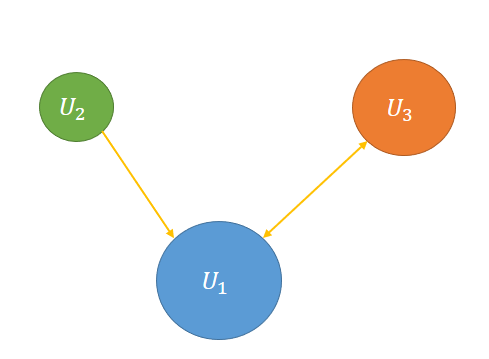
\includegraphics{D:/Doc-1718/Social Network Mining/Fudan-Social_Network_Mining/Doc/report(2)/report/1.png}
\caption{}
\end{figure}

\hypertarget{header-n13}{%
\subsubsection{Node Size}\label{header-n13}}

As you can see from the figure, the sizes of these three nodes are
different. We use the size information to denote the \emph{In-Degree}
rather than just degree. In this situation, users with more fans or
followers can have a big size.

\hypertarget{header-n16}{%
\subsubsection{Node Color}\label{header-n16}}

In this project, a quite meaningful feature of the visualization is the
color. We are not coloring the nodes randomly, in contrast, we use
different colors to represent different communities. That is, we
implement a community division algorithm through the data visualization.
We introduce the Fast Unfolding algorithm to make it. Before we
demonstrate the algorithm, we will first introduce the Community
Division task.

\hypertarget{header-n19}{%
\paragraph{Community Division}\label{header-n19}}

The main goal of the community division is to make the connection in the
samecommunity more dense while make the connection among different
communities more sparse. This can ``split'' the graph into several parts
in general based on their following and followed information.\\

\hypertarget{header-n22}{%
\paragraph{Modularity}\label{header-n22}}

Broadly speaking, modularity is the degree to which a system's
components may be separated and recombined, often with the benefit of
flexibility and variety in use. Modularity is quite an important concept
in social network mining. It describes how meaningful the community
division algorithm is. We can get the modularity as

\[Q =Σ_c  [ \frac{Σ_{in}}{2m}−(\frac{Σ_{tot}}{2m})^2]\]

If a community division is reasonable, it should have a relatively
higher modularity.

\hypertarget{header-n28}{%
\paragraph{Fast Unfolding Algorithm}\label{header-n28}}

\begin{figure}
\centering
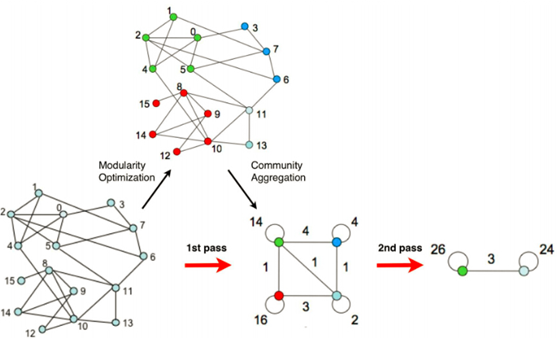
\includegraphics{D:/Doc-1718/Social Network Mining/Fudan-Social_Network_Mining/Doc/report(2)/report/2.png}
\caption{}
\end{figure}

We will illustrate the algorithm as following steps.

\begin{enumerate}
\def\labelenumi{\arabic{enumi}.}
\item
  Initialization\\

  Just make all the nodes belonging to different communities. That is,
  if we have N nodes, we have N communities initially.
\item
  Modularity Optimization

  For each node, try to divide each point into the community where its
  neighboring point is located, and calculate the degree of module at
  this point. Judging whether or not the modularity before and after the
  division is increased, if it is yes, then accept this division.
\item
  Community Aggregation

  This is the core of the algorithm. In this step, we will turn all the
  nodes in a same community into one new big node. 
\item
  Iteration

  Iterate the algorithm until the directed graph does not change.
\end{enumerate}

Using such algorithms and all the methods above, we can get the Data
Visualization result as follows:

\begin{figure}
\centering
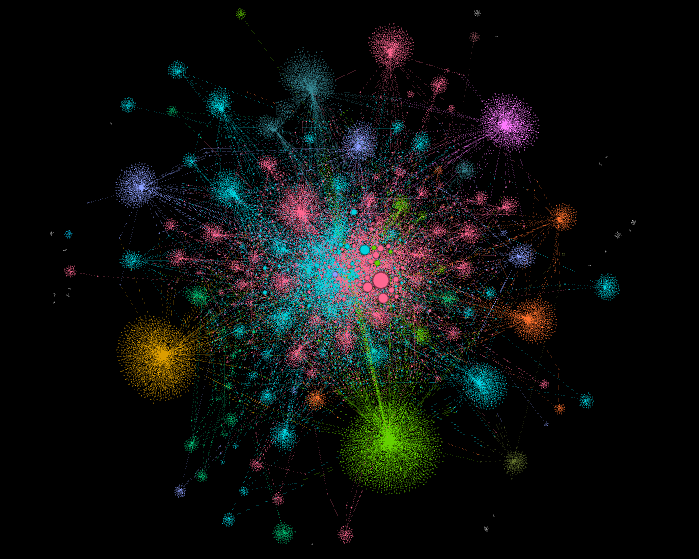
\includegraphics{D:/Doc-1718/Social Network Mining/Fudan-Social_Network_Mining/Doc/report(2)/report/3.png}
\caption{}
\end{figure}

And

\begin{figure}
\centering
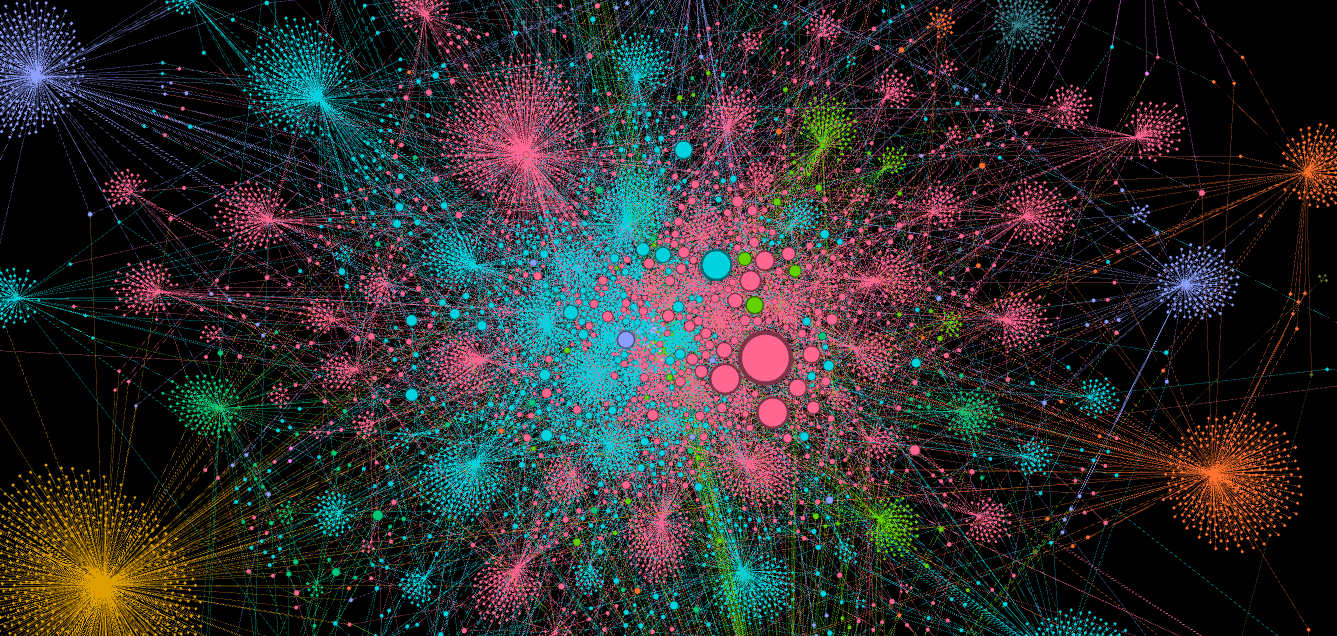
\includegraphics{D:/Doc-1718/Social Network Mining/Fudan-Social_Network_Mining/Doc/report(2)/report/5.png}
\caption{}
\end{figure}

Different colors denote different community. And we can know that the
biggest pink node in the middle has the most followers.

\begin{figure}
\centering
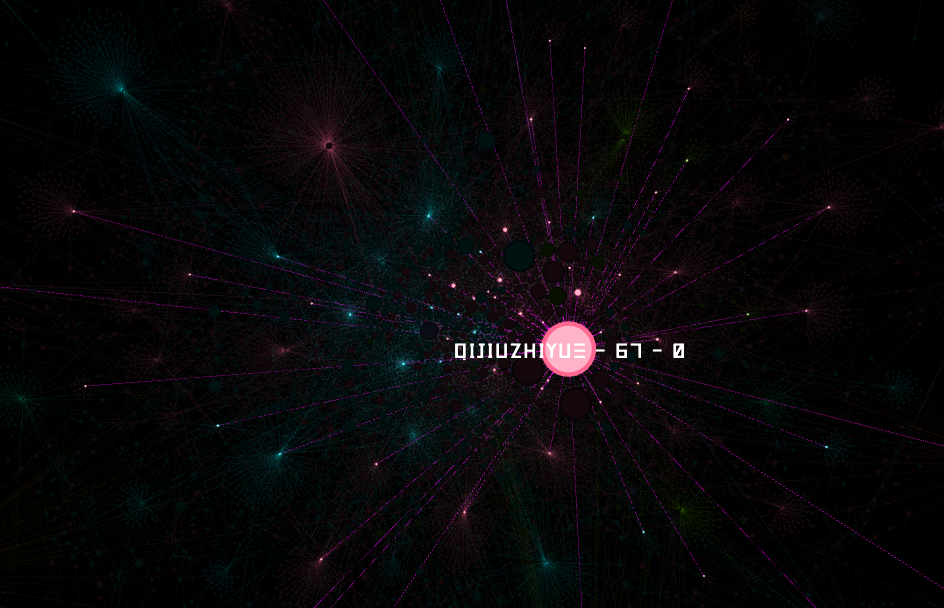
\includegraphics{D:/Doc-1718/Social Network Mining/Fudan-Social_Network_Mining/Doc/report(2)/report/6.png}
\caption{}
\end{figure}

Zoom in, we can find the user's information: user's ID, number of
followers and number of following. Besides, we highlight all the related
nodes for ease of observation.

\begin{figure}
\centering
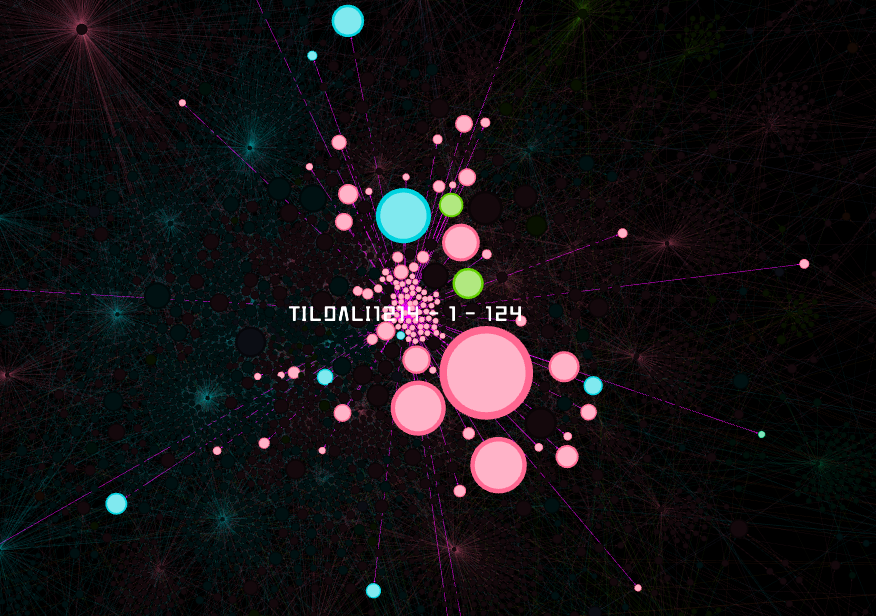
\includegraphics{D:/Doc-1718/Social Network Mining/Fudan-Social_Network_Mining/Doc/report(2)/report/4.png}
\caption{}
\end{figure}

\hypertarget{header-n72}{%
\subsection{Content-based Recommender System}\label{header-n72}}

The basis of the content-based recommendation system is that the user's
interests should match the description of the system's recommended
items. In other words, the more similar the user's interest is to the
description of the item, the more interested the user may be in the
recommended item. The content-based recommendation system achieves this
by measuring the similarity between the description of a project and the
user's personal information. The higher the similarity, the greater the
chance of the project being recommended.

We use some algorithms to embed the information of the movie and the
user's information in the same semantic space.

\hypertarget{header-n77}{%
\subsubsection{Movie Information Embedding}\label{header-n77}}

Specifically, the embedded movie vector consists of provided movie
information. We have adopted information including the movie's
publication time, ratings, screenwriters, directors, and actors.

In particular, in this project, \textbf{we proposed an original method
of embedding actors and directors in Low-dimensional vector space.} We
label both the director and the actor as artists, build an adjacency
matrix from the number of movies they have worked with, and then use the
SVD matrix decomposition to get a low-end matrix. This method not only
greatly reduces the dimension, facilitates subsequent calculations, but
also has certain semantic information embedded, which is a more reliable
method.

As the saying goes, things are gathered together and people are divided
into groups. We know that often-co-directed directors and actors may
have similar film styles. For example, the actors often appearing in
Qiong Yao's TV series may have similar artistic styles and they all like
to play soap operas. And the audience may be similar to their
preferences.

\textbf{This algorithm's inspiration comes from the word2vec algorithm.}
In the word2vec algorithm, semantically similar words are closer in
semantic space. Considering the following sentences:

\begin{itemize}
\item
  The tiny \textbf{} is so cute!
\end{itemize}

We will easily think of cat, puppy, dog, etc according to semantic
environment. And it can be proved as the Bing search result as below.

\begin{figure}
\centering
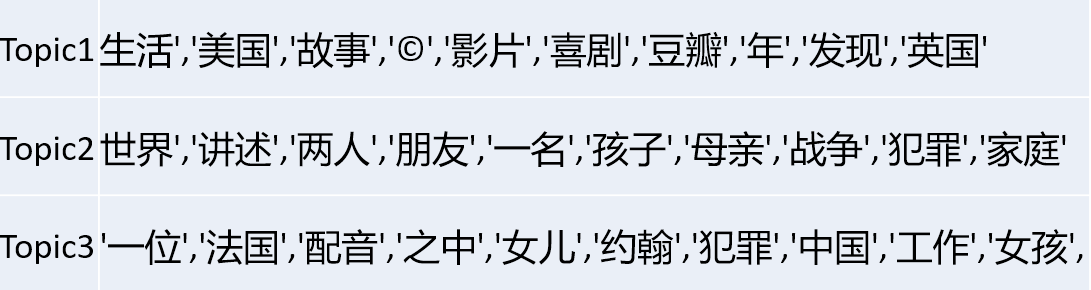
\includegraphics{D:/Doc-1718/Social Network Mining/Fudan-Social_Network_Mining/Doc/report(2)/report/7.png}
\caption{}
\end{figure}

So in the movie situation, considering the following artists:

\begin{itemize}
\item
  Tim Burton, Johnny Deep,
\item
  Daniel Radcliffe, Alan Rickman, JK Rowling.
\item
  Fan Bingbing,Zhao Wei,Su Youpeng
\end{itemize}

You might think of Helena Bonham Carter, Emma Watson, Lin Xinru
respectively. And you will never think of a Chinese actor in the first
movie environment just like you will never think of a word like
''bottle'' in the ''The tiny XXX is so cute!'' semantic environment.
Then environment entails the information! Therefore, in word2vec
algorithm, we will use the words around a particular word as the
"environment" to train the word embedding model. And in the "movie
environment", we believe the co-operation entails the environment. We
will build a "Co-operation matrix" \(M\) like below.

\begin{longtable}[]{@{}llll@{}}
\toprule
Co-operation Matrix & Tim Burton & Johnny Deep & Helena
Carter\tabularnewline
\midrule
\endhead
Tim Burton & 16 & 9 & 7\tabularnewline
Johnny Deep & 9 & 17 & 8\tabularnewline
Helena Carter & 7 & 8 & 15\tabularnewline
\bottomrule
\end{longtable}

If we have 10000 artists in total, we can have a such 10000 *10000
dimension "Co-operation matrix". And then we can SVD the matrix:

\[M = U\times S\times V\]

We will choose the top n (here 100) important dimension of all U,S,V
matrix to get off the noise as the figure shows. We denote them as
\(U',S',V'\) respectively. We will rebuild the M matrix.

\[U'\times S'\times V' = M'\]

In this situation, each \textbf{artist can be represented by a
100-dimension vector.}

\[v_{artist_{i}} = M'_{row_{i}}\]

And finally, we have

\[v_{movie_i} = cat(v_{artist_i},v_{rating_i}, v_{date_i},...)\]

In the experiment, we selected all actors (about 2,000) who performed
more than 8 times in 10,000 movies and established such a ``cooperation
matrix'' and then reduced it to 100 dimensions through PCA. This gives
each artist's expression. Finally, we use the TSNE algorithm to reduce
the matrix to 2 dimensions and visualize it. As can be seen in the
figure below, like the semantic space of word2vec, the low-dimensional
representation of our cooperation matrix dimension reduction can indeed
express a good cooperation relationship.

\begin{figure}
\centering
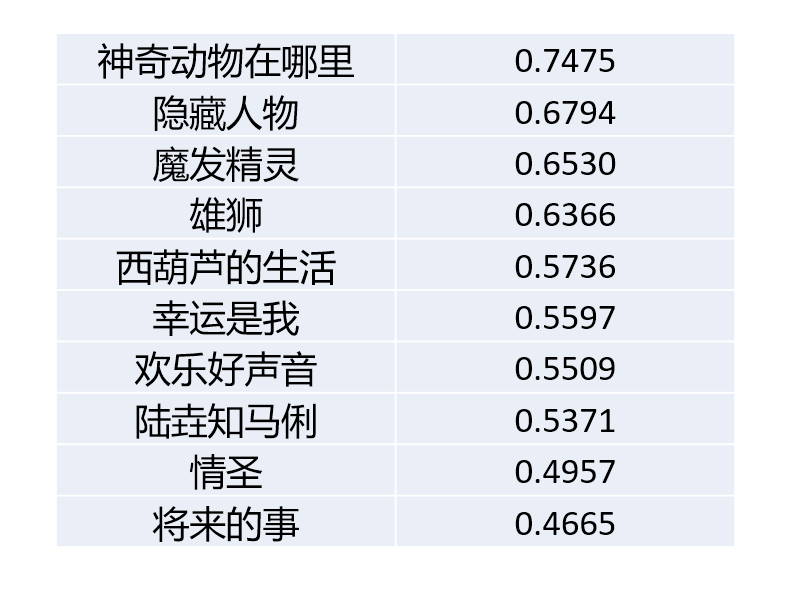
\includegraphics{D:/Doc-1718/Social Network Mining/Fudan-Social_Network_Mining/Doc/report(2)/report/8.png}
\caption{}
\end{figure}

As shown in the figure, the red region is basically a Japanese artists
community, the blue region is for Chinese artists, and the yellow one is
mainly a European and American region.

\hypertarget{header-n152}{%
\subsubsection{User Information Embedding}\label{header-n152}}

For every user, we have their rating information. We can suppose that
they love those movies which they rate them as 5 score. So we can use
all the movies they love to represent them. In this situation, we will
denote the user embedding vector as the average of their 5-score movies'
embedding vector.

\[v_{user} = \dfrac{1}{n}\sum v_{movie_{5-score}}\]

We can use this method to build the users' denoting.

\end{document}
